
\section{Experimental Protocol}\label{sec:DPR500_protocol}

% \todo[inline]{The image here is probably my best water cavitation of water image showing rare events on the threshold of cavitation.
% Greater snowstorms can be found for higher pressure but this illustrates the threshold fairly nicely - see emulsion chapter. This is 70db on the amplifier. 
% I have recorded the beam plot for this power but have yet to process this into an image that overlays the plot.
% }
% \todo[inline]{I still have a sense of so-what with these images. 
% They seem only interesting as a stepping stone as indicated in intro to ch. 6.}




\subsection{Introduction}



\subsection{Generation of the two pulses}
\subsubsection{Imaging wave}
The imaging wave is generated from a custom ordered Panemetrics \unit{20}\mega\hertz\
transducer.
The pulse/receive electronics is controlled 
with a \JsrUltrasonics \DPR500 dual pulser-receiver
with a \RPL2 pulser-receiver.
The imaging voltage was \unit{300}\volt\ and the combined imaging gain 
of the pre-amplifier and \DPR500 was \unit{50}dB.
To help reduce the contribution of the direct transmit/forward scatter of
the driving wave, a high pass filter (-\unit{3}dB at \unit{7.5}\mega\hertz)
was used.

\subsubsection{Driving wave}
The driving wave was generated from an  Analogic 2045 arbitrary waveform generator.
The input voltage was a sinusoid of frequency \unit{0.5}\mega\hertz\ 
truncated to be 10 cycles in duration. 
The output of Analogic was input into a Tomco power-generator (gain of \unit{50}dB)
which drove a \unit{0.5}\mega\hertz\ ... transducer.

\subsubsection{Controlling the timing of the two waves}
An Agilent  33220A is controlled by LAN connection.  Its role is trigged by the computer to produce a sine burst of 10 cycles.  The gate to the tomco and the analogic is conneted to the sync out.  The output is connected to the RF in on the Tomco

The analogic is to provide a delayed pulse for the \DPR500.  The reason this pulser is used rather than the Thandars or the agilent is because it has a much faster clock.  The other generators are not usable because the gitter is of order 50ns  ruining the averages.  The gitter from the analogic is nearer 5-10ns.  Its output goes to trigger the scope and to the sunc of the \DPR500.  The scope is triggered from this input so that the time recorded is genuinly a pulse-echo-time.


The \DPR500 is controlled via serial connection.  It controls the imaging spike.

The scope is controlled by LAN. Waveforms are grabbed directly from the scope.


%When imaged by the high-frequency wave the phase of the low frequency
%wave will manifest itself as a function of depth.



%The two pulses transducers need to have a common focus and we wish to
%interrogate all phase relationships between the two waves.
%This is most easily achieved by
%In this experimental arrangement the firing of the two pulses is co-ordinated so that the waves meet at
%their common focus at the same time.
%As they pass through each other at twice the speed of sound the two waves will pass through all
%possible phases.
%When imaged by the high-frequency wave the phase of the low frequency
%wave will manifest itself as a
%function of depth.
%(If this is not clear then \figref{pulses} in \secref{computational}
%may help.) 



%The limited bandwidth of the high-frequency transducer is relied upon
%to filter out the direct transmit of the low-frequency wave.


\subsection{The Experimental container}
The experiment is carried out with a experimental chamber built by Mr Craig ...
The dimensions are drawn in \figref{chamber_drawing}
and a photo is seen in \figref{chamber_photo}.
A water bath is provided for both the driving and imaging transducers,
both such that the geometric focus is coincident in the middle of central,
reaction chamber.
the central chamber can be closed with a plastic acoustic medium.
However,
in this experiment no such division was made.


\subsection{Summary of arrangement}
The full arrangement is given in \figref{arrangement}.



%\subsection{The characterisation of the nucleated bubbles}\label{sec:WE:characterisation}


\subsection{The experimental volume}

Beamplot goes here.

\subsubsection{Generation of Bubbles}

\subsubsection{Assumptions made}





%When I high frequency wave - the imaging wave -
%is incident 
%It does so indirectly.
%First, the 
%It was shown that when a bubble is shrunk, 
%even temporarily, 
%that the resonance frequency of the bubble increases.
%The bubble's response to a high frequency imaging wave can be tuned by varying the phase of% the bubble's cycle at which the bubble is incident.
%The phase of the bubble, in turn,
%may be controlled by a second, lower frequency wave.
%When the phase of the low frequency wave - the driving wave - 
%is such that the bubble is temporarily shrunk,
%the resonance frequency of the bubble temporarily increases.
%If a short high frequency pulse is incident on the b
%The bubble's response to a second, high frequency imaging wave can be tuned by varying the phase relationship between the two waves.




\section{A motivating  example}\label{sec:WE:motivating_ex}

\begin{figure}[t]%
  \centering
  \subfloat[1st pulse - 100]{
    \label{fig:av:108:100_ex:first}
    % GNUPLOT: LaTeX picture with Postscript
\begingroup
  \makeatletter
  \providecommand\color[2][]{%
    \GenericError{(gnuplot) \space\space\space\@spaces}{%
      Package color not loaded in conjunction with
      terminal option `colourtext'%
    }{See the gnuplot documentation for explanation.%
    }{Either use 'blacktext' in gnuplot or load the package
      color.sty in LaTeX.}%
    \renewcommand\color[2][]{}%
  }%
  \providecommand\includegraphics[2][]{%
    \GenericError{(gnuplot) \space\space\space\@spaces}{%
      Package graphicx or graphics not loaded%
    }{See the gnuplot documentation for explanation.%
    }{The gnuplot epslatex terminal needs graphicx.sty or graphics.sty.}%
    \renewcommand\includegraphics[2][]{}%
  }%
  \providecommand\rotatebox[2]{#2}%
  \@ifundefined{ifGPcolor}{%
    \newif\ifGPcolor
    \GPcolortrue
  }{}%
  \@ifundefined{ifGPblacktext}{%
    \newif\ifGPblacktext
    \GPblacktexttrue
  }{}%
  % define a \g@addto@macro without @ in the name:
  \let\gplgaddtomacro\g@addto@macro
  % define empty templates for all commands taking text:
  \gdef\gplbacktext{}%
  \gdef\gplfronttext{}%
  \makeatother
  \ifGPblacktext
    % no textcolor at all
    \def\colorrgb#1{}%
    \def\colorgray#1{}%
  \else
    % gray or color?
    \ifGPcolor
      \def\colorrgb#1{\color[rgb]{#1}}%
      \def\colorgray#1{\color[gray]{#1}}%
      \expandafter\def\csname LTw\endcsname{\color{white}}%
      \expandafter\def\csname LTb\endcsname{\color{black}}%
      \expandafter\def\csname LTa\endcsname{\color{black}}%
      \expandafter\def\csname LT0\endcsname{\color[rgb]{1,0,0}}%
      \expandafter\def\csname LT1\endcsname{\color[rgb]{0,1,0}}%
      \expandafter\def\csname LT2\endcsname{\color[rgb]{0,0,1}}%
      \expandafter\def\csname LT3\endcsname{\color[rgb]{1,0,1}}%
      \expandafter\def\csname LT4\endcsname{\color[rgb]{0,1,1}}%
      \expandafter\def\csname LT5\endcsname{\color[rgb]{1,1,0}}%
      \expandafter\def\csname LT6\endcsname{\color[rgb]{0,0,0}}%
      \expandafter\def\csname LT7\endcsname{\color[rgb]{1,0.3,0}}%
      \expandafter\def\csname LT8\endcsname{\color[rgb]{0.5,0.5,0.5}}%
    \else
      % gray
      \def\colorrgb#1{\color{black}}%
      \def\colorgray#1{\color[gray]{#1}}%
      \expandafter\def\csname LTw\endcsname{\color{white}}%
      \expandafter\def\csname LTb\endcsname{\color{black}}%
      \expandafter\def\csname LTa\endcsname{\color{black}}%
      \expandafter\def\csname LT0\endcsname{\color{black}}%
      \expandafter\def\csname LT1\endcsname{\color{black}}%
      \expandafter\def\csname LT2\endcsname{\color{black}}%
      \expandafter\def\csname LT3\endcsname{\color{black}}%
      \expandafter\def\csname LT4\endcsname{\color{black}}%
      \expandafter\def\csname LT5\endcsname{\color{black}}%
      \expandafter\def\csname LT6\endcsname{\color{black}}%
      \expandafter\def\csname LT7\endcsname{\color{black}}%
      \expandafter\def\csname LT8\endcsname{\color{black}}%
    \fi
  \fi
  \setlength{\unitlength}{0.0500bp}%
  \begin{picture}(2880.00,2520.00)%
    \gplgaddtomacro\gplbacktext{%
      \csname LTb\endcsname%
      \put(-119,782){\makebox(0,0)[r]{\strut{}-1}}%
      \put(-119,1040){\makebox(0,0)[r]{\strut{}-0.5}}%
      \put(-119,1298){\makebox(0,0)[r]{\strut{} 0}}%
      \put(-119,1556){\makebox(0,0)[r]{\strut{} 0.5}}%
      \put(-119,1814){\makebox(0,0)[r]{\strut{} 1}}%
      \put(-119,2072){\makebox(0,0)[r]{\strut{} 1.5}}%
      \put(-119,2330){\makebox(0,0)[r]{\strut{} 2}}%
      \put(13,484){\makebox(0,0){\strut{} 0}}%
      \put(421,484){\makebox(0,0){\strut{} 5}}%
      \put(828,484){\makebox(0,0){\strut{} 10}}%
      \put(1236,484){\makebox(0,0){\strut{} 15}}%
      \put(1643,484){\makebox(0,0){\strut{} 20}}%
      \put(2051,484){\makebox(0,0){\strut{} 25}}%
      \put(2458,484){\makebox(0,0){\strut{} 30}}%
      \put(2866,484){\makebox(0,0){\strut{} 35}}%
      \put(-889,1590){\rotatebox{-270}{\makebox(0,0){\strut{}voltage (V)}}}%
      \put(1439,154){\makebox(0,0){\strut{}time ($\mu$ s)}}%
    }%
    \gplgaddtomacro\gplfronttext{%
      \csname LTb\endcsname%
      \put(2381,2303){\makebox(0,0)[r]{\strut{}1-$\sigma$}}%
      \csname LTb\endcsname%
      \put(2381,2083){\makebox(0,0)[r]{\strut{}av.}}%
    }%
    \gplbacktext
    \put(0,0){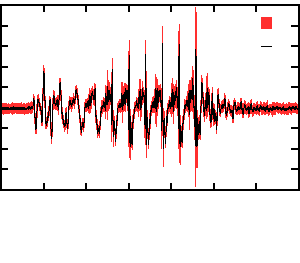
\includegraphics{voltage_0_108_gap_between_pulses_100_no_imaging_av_with_sd_means1_large}}%
    \gplfronttext
  \end{picture}%
\endgroup
}
 \quad
  \subfloat[2nd pulse - 100]{
    \label{fig:av:108:100_ex:second}
    % GNUPLOT: LaTeX picture with Postscript
\begingroup
  \makeatletter
  \providecommand\color[2][]{%
    \GenericError{(gnuplot) \space\space\space\@spaces}{%
      Package color not loaded in conjunction with
      terminal option `colourtext'%
    }{See the gnuplot documentation for explanation.%
    }{Either use 'blacktext' in gnuplot or load the package
      color.sty in LaTeX.}%
    \renewcommand\color[2][]{}%
  }%
  \providecommand\includegraphics[2][]{%
    \GenericError{(gnuplot) \space\space\space\@spaces}{%
      Package graphicx or graphics not loaded%
    }{See the gnuplot documentation for explanation.%
    }{The gnuplot epslatex terminal needs graphicx.sty or graphics.sty.}%
    \renewcommand\includegraphics[2][]{}%
  }%
  \providecommand\rotatebox[2]{#2}%
  \@ifundefined{ifGPcolor}{%
    \newif\ifGPcolor
    \GPcolortrue
  }{}%
  \@ifundefined{ifGPblacktext}{%
    \newif\ifGPblacktext
    \GPblacktexttrue
  }{}%
  % define a \g@addto@macro without @ in the name:
  \let\gplgaddtomacro\g@addto@macro
  % define empty templates for all commands taking text:
  \gdef\gplbacktext{}%
  \gdef\gplfronttext{}%
  \makeatother
  \ifGPblacktext
    % no textcolor at all
    \def\colorrgb#1{}%
    \def\colorgray#1{}%
  \else
    % gray or color?
    \ifGPcolor
      \def\colorrgb#1{\color[rgb]{#1}}%
      \def\colorgray#1{\color[gray]{#1}}%
      \expandafter\def\csname LTw\endcsname{\color{white}}%
      \expandafter\def\csname LTb\endcsname{\color{black}}%
      \expandafter\def\csname LTa\endcsname{\color{black}}%
      \expandafter\def\csname LT0\endcsname{\color[rgb]{1,0,0}}%
      \expandafter\def\csname LT1\endcsname{\color[rgb]{0,1,0}}%
      \expandafter\def\csname LT2\endcsname{\color[rgb]{0,0,1}}%
      \expandafter\def\csname LT3\endcsname{\color[rgb]{1,0,1}}%
      \expandafter\def\csname LT4\endcsname{\color[rgb]{0,1,1}}%
      \expandafter\def\csname LT5\endcsname{\color[rgb]{1,1,0}}%
      \expandafter\def\csname LT6\endcsname{\color[rgb]{0,0,0}}%
      \expandafter\def\csname LT7\endcsname{\color[rgb]{1,0.3,0}}%
      \expandafter\def\csname LT8\endcsname{\color[rgb]{0.5,0.5,0.5}}%
    \else
      % gray
      \def\colorrgb#1{\color{black}}%
      \def\colorgray#1{\color[gray]{#1}}%
      \expandafter\def\csname LTw\endcsname{\color{white}}%
      \expandafter\def\csname LTb\endcsname{\color{black}}%
      \expandafter\def\csname LTa\endcsname{\color{black}}%
      \expandafter\def\csname LT0\endcsname{\color{black}}%
      \expandafter\def\csname LT1\endcsname{\color{black}}%
      \expandafter\def\csname LT2\endcsname{\color{black}}%
      \expandafter\def\csname LT3\endcsname{\color{black}}%
      \expandafter\def\csname LT4\endcsname{\color{black}}%
      \expandafter\def\csname LT5\endcsname{\color{black}}%
      \expandafter\def\csname LT6\endcsname{\color{black}}%
      \expandafter\def\csname LT7\endcsname{\color{black}}%
      \expandafter\def\csname LT8\endcsname{\color{black}}%
    \fi
  \fi
  \setlength{\unitlength}{0.0500bp}%
  \begin{picture}(2880.00,2520.00)%
    \gplgaddtomacro\gplbacktext{%
      \csname LTb\endcsname%
      \put(-119,704){\makebox(0,0)[r]{\strut{}}}%
      \put(-119,926){\makebox(0,0)[r]{\strut{}}}%
      \put(-119,1147){\makebox(0,0)[r]{\strut{}}}%
      \put(-119,1369){\makebox(0,0)[r]{\strut{}}}%
      \put(-119,1590){\makebox(0,0)[r]{\strut{}}}%
      \put(-119,1812){\makebox(0,0)[r]{\strut{}}}%
      \put(-119,2033){\makebox(0,0)[r]{\strut{}}}%
      \put(-119,2255){\makebox(0,0)[r]{\strut{}}}%
      \put(-119,2476){\makebox(0,0)[r]{\strut{}}}%
      \put(13,484){\makebox(0,0){\strut{} 0}}%
      \put(421,484){\makebox(0,0){\strut{} 5}}%
      \put(828,484){\makebox(0,0){\strut{} 10}}%
      \put(1236,484){\makebox(0,0){\strut{} 15}}%
      \put(1643,484){\makebox(0,0){\strut{} 20}}%
      \put(2051,484){\makebox(0,0){\strut{} 25}}%
      \put(2458,484){\makebox(0,0){\strut{} 30}}%
      \put(2866,484){\makebox(0,0){\strut{} 35}}%
      \put(1439,154){\makebox(0,0){\strut{}time ($\mu$ s)}}%
    }%
    \gplgaddtomacro\gplfronttext{%
      \csname LTb\endcsname%
      \put(2381,2303){\makebox(0,0)[r]{\strut{}1-$\sigma$}}%
      \csname LTb\endcsname%
      \put(2381,2083){\makebox(0,0)[r]{\strut{}av.}}%
    }%
    \gplbacktext
    \put(0,0){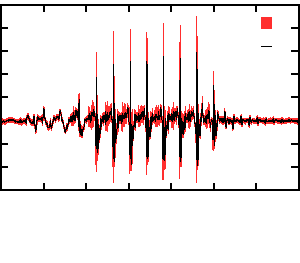
\includegraphics{voltage_0_108_gap_between_pulses_100_no_imaging_av_with_sd_means2_large}}%
    \gplfronttext
  \end{picture}%
\endgroup
}\\
 \subfloat[1st pulse - 12000]{
    \label{fig:av:108:12000_ex:first}
    % GNUPLOT: LaTeX picture with Postscript
\begingroup
  \makeatletter
  \providecommand\color[2][]{%
    \GenericError{(gnuplot) \space\space\space\@spaces}{%
      Package color not loaded in conjunction with
      terminal option `colourtext'%
    }{See the gnuplot documentation for explanation.%
    }{Either use 'blacktext' in gnuplot or load the package
      color.sty in LaTeX.}%
    \renewcommand\color[2][]{}%
  }%
  \providecommand\includegraphics[2][]{%
    \GenericError{(gnuplot) \space\space\space\@spaces}{%
      Package graphicx or graphics not loaded%
    }{See the gnuplot documentation for explanation.%
    }{The gnuplot epslatex terminal needs graphicx.sty or graphics.sty.}%
    \renewcommand\includegraphics[2][]{}%
  }%
  \providecommand\rotatebox[2]{#2}%
  \@ifundefined{ifGPcolor}{%
    \newif\ifGPcolor
    \GPcolortrue
  }{}%
  \@ifundefined{ifGPblacktext}{%
    \newif\ifGPblacktext
    \GPblacktexttrue
  }{}%
  % define a \g@addto@macro without @ in the name:
  \let\gplgaddtomacro\g@addto@macro
  % define empty templates for all commands taking text:
  \gdef\gplbacktext{}%
  \gdef\gplfronttext{}%
  \makeatother
  \ifGPblacktext
    % no textcolor at all
    \def\colorrgb#1{}%
    \def\colorgray#1{}%
  \else
    % gray or color?
    \ifGPcolor
      \def\colorrgb#1{\color[rgb]{#1}}%
      \def\colorgray#1{\color[gray]{#1}}%
      \expandafter\def\csname LTw\endcsname{\color{white}}%
      \expandafter\def\csname LTb\endcsname{\color{black}}%
      \expandafter\def\csname LTa\endcsname{\color{black}}%
      \expandafter\def\csname LT0\endcsname{\color[rgb]{1,0,0}}%
      \expandafter\def\csname LT1\endcsname{\color[rgb]{0,1,0}}%
      \expandafter\def\csname LT2\endcsname{\color[rgb]{0,0,1}}%
      \expandafter\def\csname LT3\endcsname{\color[rgb]{1,0,1}}%
      \expandafter\def\csname LT4\endcsname{\color[rgb]{0,1,1}}%
      \expandafter\def\csname LT5\endcsname{\color[rgb]{1,1,0}}%
      \expandafter\def\csname LT6\endcsname{\color[rgb]{0,0,0}}%
      \expandafter\def\csname LT7\endcsname{\color[rgb]{1,0.3,0}}%
      \expandafter\def\csname LT8\endcsname{\color[rgb]{0.5,0.5,0.5}}%
    \else
      % gray
      \def\colorrgb#1{\color{black}}%
      \def\colorgray#1{\color[gray]{#1}}%
      \expandafter\def\csname LTw\endcsname{\color{white}}%
      \expandafter\def\csname LTb\endcsname{\color{black}}%
      \expandafter\def\csname LTa\endcsname{\color{black}}%
      \expandafter\def\csname LT0\endcsname{\color{black}}%
      \expandafter\def\csname LT1\endcsname{\color{black}}%
      \expandafter\def\csname LT2\endcsname{\color{black}}%
      \expandafter\def\csname LT3\endcsname{\color{black}}%
      \expandafter\def\csname LT4\endcsname{\color{black}}%
      \expandafter\def\csname LT5\endcsname{\color{black}}%
      \expandafter\def\csname LT6\endcsname{\color{black}}%
      \expandafter\def\csname LT7\endcsname{\color{black}}%
      \expandafter\def\csname LT8\endcsname{\color{black}}%
    \fi
  \fi
  \setlength{\unitlength}{0.0500bp}%
  \begin{picture}(2880.00,2520.00)%
    \gplgaddtomacro\gplbacktext{%
      \csname LTb\endcsname%
      \put(-119,782){\makebox(0,0)[r]{\strut{}-1}}%
      \put(-119,1040){\makebox(0,0)[r]{\strut{}-0.5}}%
      \put(-119,1298){\makebox(0,0)[r]{\strut{} 0}}%
      \put(-119,1556){\makebox(0,0)[r]{\strut{} 0.5}}%
      \put(-119,1814){\makebox(0,0)[r]{\strut{} 1}}%
      \put(-119,2072){\makebox(0,0)[r]{\strut{} 1.5}}%
      \put(-119,2330){\makebox(0,0)[r]{\strut{} 2}}%
      \put(13,484){\makebox(0,0){\strut{} 0}}%
      \put(421,484){\makebox(0,0){\strut{} 5}}%
      \put(828,484){\makebox(0,0){\strut{} 10}}%
      \put(1236,484){\makebox(0,0){\strut{} 15}}%
      \put(1643,484){\makebox(0,0){\strut{} 20}}%
      \put(2051,484){\makebox(0,0){\strut{} 25}}%
      \put(2458,484){\makebox(0,0){\strut{} 30}}%
      \put(2866,484){\makebox(0,0){\strut{} 35}}%
      \put(-889,1590){\rotatebox{-270}{\makebox(0,0){\strut{}voltage (V)}}}%
      \put(1439,154){\makebox(0,0){\strut{}time ($\mu$ s)}}%
    }%
    \gplgaddtomacro\gplfronttext{%
      \csname LTb\endcsname%
      \put(2381,2303){\makebox(0,0)[r]{\strut{}1-$\sigma$}}%
      \csname LTb\endcsname%
      \put(2381,2083){\makebox(0,0)[r]{\strut{}av.}}%
    }%
    \gplbacktext
    \put(0,0){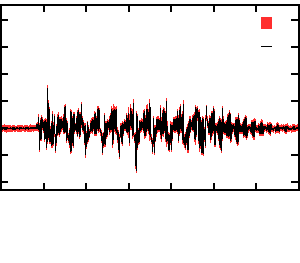
\includegraphics{voltage_0_108_gap_between_pulses_12000_no_imaging_av_with_sd_means1_large}}%
    \gplfronttext
  \end{picture}%
\endgroup
}
 \quad
  \subfloat[2nd pulse - 12000]{
    \label{fig:av:108:12000_ex:second}
    % GNUPLOT: LaTeX picture with Postscript
\begingroup
  \makeatletter
  \providecommand\color[2][]{%
    \GenericError{(gnuplot) \space\space\space\@spaces}{%
      Package color not loaded in conjunction with
      terminal option `colourtext'%
    }{See the gnuplot documentation for explanation.%
    }{Either use 'blacktext' in gnuplot or load the package
      color.sty in LaTeX.}%
    \renewcommand\color[2][]{}%
  }%
  \providecommand\includegraphics[2][]{%
    \GenericError{(gnuplot) \space\space\space\@spaces}{%
      Package graphicx or graphics not loaded%
    }{See the gnuplot documentation for explanation.%
    }{The gnuplot epslatex terminal needs graphicx.sty or graphics.sty.}%
    \renewcommand\includegraphics[2][]{}%
  }%
  \providecommand\rotatebox[2]{#2}%
  \@ifundefined{ifGPcolor}{%
    \newif\ifGPcolor
    \GPcolortrue
  }{}%
  \@ifundefined{ifGPblacktext}{%
    \newif\ifGPblacktext
    \GPblacktexttrue
  }{}%
  % define a \g@addto@macro without @ in the name:
  \let\gplgaddtomacro\g@addto@macro
  % define empty templates for all commands taking text:
  \gdef\gplbacktext{}%
  \gdef\gplfronttext{}%
  \makeatother
  \ifGPblacktext
    % no textcolor at all
    \def\colorrgb#1{}%
    \def\colorgray#1{}%
  \else
    % gray or color?
    \ifGPcolor
      \def\colorrgb#1{\color[rgb]{#1}}%
      \def\colorgray#1{\color[gray]{#1}}%
      \expandafter\def\csname LTw\endcsname{\color{white}}%
      \expandafter\def\csname LTb\endcsname{\color{black}}%
      \expandafter\def\csname LTa\endcsname{\color{black}}%
      \expandafter\def\csname LT0\endcsname{\color[rgb]{1,0,0}}%
      \expandafter\def\csname LT1\endcsname{\color[rgb]{0,1,0}}%
      \expandafter\def\csname LT2\endcsname{\color[rgb]{0,0,1}}%
      \expandafter\def\csname LT3\endcsname{\color[rgb]{1,0,1}}%
      \expandafter\def\csname LT4\endcsname{\color[rgb]{0,1,1}}%
      \expandafter\def\csname LT5\endcsname{\color[rgb]{1,1,0}}%
      \expandafter\def\csname LT6\endcsname{\color[rgb]{0,0,0}}%
      \expandafter\def\csname LT7\endcsname{\color[rgb]{1,0.3,0}}%
      \expandafter\def\csname LT8\endcsname{\color[rgb]{0.5,0.5,0.5}}%
    \else
      % gray
      \def\colorrgb#1{\color{black}}%
      \def\colorgray#1{\color[gray]{#1}}%
      \expandafter\def\csname LTw\endcsname{\color{white}}%
      \expandafter\def\csname LTb\endcsname{\color{black}}%
      \expandafter\def\csname LTa\endcsname{\color{black}}%
      \expandafter\def\csname LT0\endcsname{\color{black}}%
      \expandafter\def\csname LT1\endcsname{\color{black}}%
      \expandafter\def\csname LT2\endcsname{\color{black}}%
      \expandafter\def\csname LT3\endcsname{\color{black}}%
      \expandafter\def\csname LT4\endcsname{\color{black}}%
      \expandafter\def\csname LT5\endcsname{\color{black}}%
      \expandafter\def\csname LT6\endcsname{\color{black}}%
      \expandafter\def\csname LT7\endcsname{\color{black}}%
      \expandafter\def\csname LT8\endcsname{\color{black}}%
    \fi
  \fi
  \setlength{\unitlength}{0.0500bp}%
  \begin{picture}(2880.00,2520.00)%
    \gplgaddtomacro\gplbacktext{%
      \csname LTb\endcsname%
      \put(-119,782){\makebox(0,0)[r]{\strut{}}}%
      \put(-119,1040){\makebox(0,0)[r]{\strut{}}}%
      \put(-119,1298){\makebox(0,0)[r]{\strut{}}}%
      \put(-119,1556){\makebox(0,0)[r]{\strut{}}}%
      \put(-119,1814){\makebox(0,0)[r]{\strut{}}}%
      \put(-119,2072){\makebox(0,0)[r]{\strut{}}}%
      \put(-119,2330){\makebox(0,0)[r]{\strut{}}}%
      \put(13,484){\makebox(0,0){\strut{} 0}}%
      \put(421,484){\makebox(0,0){\strut{} 5}}%
      \put(828,484){\makebox(0,0){\strut{} 10}}%
      \put(1236,484){\makebox(0,0){\strut{} 15}}%
      \put(1643,484){\makebox(0,0){\strut{} 20}}%
      \put(2051,484){\makebox(0,0){\strut{} 25}}%
      \put(2458,484){\makebox(0,0){\strut{} 30}}%
      \put(2866,484){\makebox(0,0){\strut{} 35}}%
      \put(1439,154){\makebox(0,0){\strut{}time ($\mu$ s)}}%
    }%
    \gplgaddtomacro\gplfronttext{%
      \csname LTb\endcsname%
      \put(2381,2303){\makebox(0,0)[r]{\strut{}1-$\sigma$}}%
      \csname LTb\endcsname%
      \put(2381,2083){\makebox(0,0)[r]{\strut{}av.}}%
    }%
    \gplbacktext
    \put(0,0){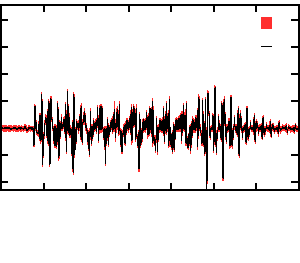
\includegraphics{voltage_0_108_gap_between_pulses_12000_no_imaging_av_with_sd_means2_large}}%
    \gplfronttext
  \end{picture}%
\endgroup
}\\
  \subfloat[2nd pulse - 12000]{
    \label{fig:av:108:12000_ex:sub}
    % GNUPLOT: LaTeX picture with Postscript
\begingroup
  \makeatletter
  \providecommand\color[2][]{%
    \GenericError{(gnuplot) \space\space\space\@spaces}{%
      Package color not loaded in conjunction with
      terminal option `colourtext'%
    }{See the gnuplot documentation for explanation.%
    }{Either use 'blacktext' in gnuplot or load the package
      color.sty in LaTeX.}%
    \renewcommand\color[2][]{}%
  }%
  \providecommand\includegraphics[2][]{%
    \GenericError{(gnuplot) \space\space\space\@spaces}{%
      Package graphicx or graphics not loaded%
    }{See the gnuplot documentation for explanation.%
    }{The gnuplot epslatex terminal needs graphicx.sty or graphics.sty.}%
    \renewcommand\includegraphics[2][]{}%
  }%
  \providecommand\rotatebox[2]{#2}%
  \@ifundefined{ifGPcolor}{%
    \newif\ifGPcolor
    \GPcolortrue
  }{}%
  \@ifundefined{ifGPblacktext}{%
    \newif\ifGPblacktext
    \GPblacktexttrue
  }{}%
  % define a \g@addto@macro without @ in the name:
  \let\gplgaddtomacro\g@addto@macro
  % define empty templates for all commands taking text:
  \gdef\gplbacktext{}%
  \gdef\gplfronttext{}%
  \makeatother
  \ifGPblacktext
    % no textcolor at all
    \def\colorrgb#1{}%
    \def\colorgray#1{}%
  \else
    % gray or color?
    \ifGPcolor
      \def\colorrgb#1{\color[rgb]{#1}}%
      \def\colorgray#1{\color[gray]{#1}}%
      \expandafter\def\csname LTw\endcsname{\color{white}}%
      \expandafter\def\csname LTb\endcsname{\color{black}}%
      \expandafter\def\csname LTa\endcsname{\color{black}}%
      \expandafter\def\csname LT0\endcsname{\color[rgb]{1,0,0}}%
      \expandafter\def\csname LT1\endcsname{\color[rgb]{0,1,0}}%
      \expandafter\def\csname LT2\endcsname{\color[rgb]{0,0,1}}%
      \expandafter\def\csname LT3\endcsname{\color[rgb]{1,0,1}}%
      \expandafter\def\csname LT4\endcsname{\color[rgb]{0,1,1}}%
      \expandafter\def\csname LT5\endcsname{\color[rgb]{1,1,0}}%
      \expandafter\def\csname LT6\endcsname{\color[rgb]{0,0,0}}%
      \expandafter\def\csname LT7\endcsname{\color[rgb]{1,0.3,0}}%
      \expandafter\def\csname LT8\endcsname{\color[rgb]{0.5,0.5,0.5}}%
    \else
      % gray
      \def\colorrgb#1{\color{black}}%
      \def\colorgray#1{\color[gray]{#1}}%
      \expandafter\def\csname LTw\endcsname{\color{white}}%
      \expandafter\def\csname LTb\endcsname{\color{black}}%
      \expandafter\def\csname LTa\endcsname{\color{black}}%
      \expandafter\def\csname LT0\endcsname{\color{black}}%
      \expandafter\def\csname LT1\endcsname{\color{black}}%
      \expandafter\def\csname LT2\endcsname{\color{black}}%
      \expandafter\def\csname LT3\endcsname{\color{black}}%
      \expandafter\def\csname LT4\endcsname{\color{black}}%
      \expandafter\def\csname LT5\endcsname{\color{black}}%
      \expandafter\def\csname LT6\endcsname{\color{black}}%
      \expandafter\def\csname LT7\endcsname{\color{black}}%
      \expandafter\def\csname LT8\endcsname{\color{black}}%
    \fi
  \fi
  \setlength{\unitlength}{0.0500bp}%
  \begin{picture}(2880.00,2520.00)%
    \gplgaddtomacro\gplbacktext{%
      \csname LTb\endcsname%
      \put(-119,782){\makebox(0,0)[r]{\strut{}-1}}%
      \put(-119,1040){\makebox(0,0)[r]{\strut{}-0.5}}%
      \put(-119,1298){\makebox(0,0)[r]{\strut{} 0}}%
      \put(-119,1556){\makebox(0,0)[r]{\strut{} 0.5}}%
      \put(-119,1814){\makebox(0,0)[r]{\strut{} 1}}%
      \put(-119,2072){\makebox(0,0)[r]{\strut{} 1.5}}%
      \put(-119,2330){\makebox(0,0)[r]{\strut{} 2}}%
      \put(13,484){\makebox(0,0){\strut{} 0}}%
      \put(421,484){\makebox(0,0){\strut{} 5}}%
      \put(828,484){\makebox(0,0){\strut{} 10}}%
      \put(1236,484){\makebox(0,0){\strut{} 15}}%
      \put(1643,484){\makebox(0,0){\strut{} 20}}%
      \put(2051,484){\makebox(0,0){\strut{} 25}}%
      \put(2458,484){\makebox(0,0){\strut{} 30}}%
      \put(2866,484){\makebox(0,0){\strut{} 35}}%
      \put(-889,1590){\rotatebox{-270}{\makebox(0,0){\strut{}voltage (V)}}}%
      \put(1439,154){\makebox(0,0){\strut{}time ($\mu$ s)}}%
    }%
    \gplgaddtomacro\gplfronttext{%
      \csname LTb\endcsname%
      \put(2381,2303){\makebox(0,0)[r]{\strut{}1-$\sigma$}}%
      \csname LTb\endcsname%
      \put(2381,2083){\makebox(0,0)[r]{\strut{}av.}}%
    }%
    \gplbacktext
    \put(0,0){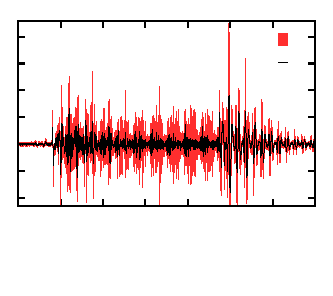
\includegraphics{voltage_0_108_gap_between_pulses_12000_no_imaging_av_with_sd_means_sub_large}}%
    \gplfronttext
  \end{picture}%
\endgroup
}\\
  \caption{
    The pressure received  by the imaging transducer when the driving wave is on but the imaging wave is off (receive-only).
    The second pulse \subref{fig:av:108:100:second} is received \unit{100}\micro\second\ after the first \subref{fig:av:108:100:first}.
    Each image is the average of 49 images, the first standard-deviation error bars are indicated.
  }
  \label{fig:av:108:100_ex}
\end{figure}



%\Figref{av:108:1000_ex:first} illustrates 

To motivate the use of water as a the cavitating medium, 
we illustrate a preliminary experiment that demonstrates the signal recieved by the high frequency transducer.
\Figref{av:108:1000} shows the pressure received by the imaging transducer when the driving wave pressure is 0.108V at the focus.

That a bubble is actually created is illustrated in 

Need to demonstrate bubble.
need to demonstrate nucleation threshold.
need to demonstrate 

%
%Is it a bubble?
%
%Qualitatively the image is similar to those generated by the computer model.
%A more detailed comparison on these lines will happen in \chapref{infer_model}.



\nlist{
  \item A bubble is transiently created at the bright regions and dissolves in the dark regions (a very short lived bubble).
\item A bubble is created and lives for the entire A-line and then dissolves/returns to its mote before being generated again in the next A-line (i.e. The lifetime of the bubble is less than the time between adjacent A-lines).
\item A bubble is created and lives for a while (see it for many A-lines).  
}
If the third of these were true then it must be explained  why the bubble cannot be seen when the driving wave is off (for example, the bubble is small).

To give an interpretation I think the following question must be answered:

\begin{sidetext}{}{Important Question}
  Is the signal backscatter from the imaging wave or forward scatter from the driving transducer or a mixture of the two?
\end{sidetext}
If the signal is just forward scatter then we are simply doing passive cavitation detection,
via an overly complicated harmonic imaging setup.
There is then no relation to the computational work done.
There is no new technology at work.
It should also be said that if this is the case then we are also using the word cavitation in its loosest sense.
We could not claim to be generating a bubble - the bubble probably does exist, but is just not visible at the pressures and frequencies used in the imaging setup.
The result would then be ``If you use a sufficiently high pressure you can pulsate a small bubble  to generate higher-frequency harmonics''.
I do not feel that this is a novel contribution.


If the signal is just back-scatter then we have a very interesting result.
It could be that the bubble is very short lived, or that the driving wave has influenced the backscatter of the imaging wave.
The second of these is the result that we are looking for, but a very short lived bubble would be interesting too.

If the signal is a combination of forward-scatter and backscatter then we need a way of separating out `interesting' backscatter from the dull forward scatter.
This issue was discussed at length in \chapref{mechanisms}.
The way to do this is to subtract an image generated when only the driving wave is present (providing the forward scatter and direct transmit)
from an image containing both waves.
Then you are left with the contribution from the imaging wave.

If the bubble is the same in both images then the forward transmit will be subtracted away.
If all the signal is removed in the subtraction then we have simply been doing harmonic imaging and therefore contributed nothing.
(I.e. pulse inversion without inverting the pulse).
If a portion of the signal is obliterated then we have the imaging wave interacting with the driving wave (the most interesting result).
The beginning of the resultant signal indicates where the bubble is located (see \chapref{mechanisms}).
If the signals are in no way obliterated then it indicates that the bubble was not the same from one pulse to the next:
it indicates that we are destroying/creating the bubbles with the driving wave.

\todo[inline]{%
The problem, therefore,  is that I cannot distinguish an interesting result (the driving wave and imaging wave interacting, or very short lived bubbles)
from a result that contributes very little (harmonic imaging).
To resolve this problem the imaging transducer needs to be able to be turned off.
However, this is not easy to do with the Cortex.
To answer these questions I need a pulse-receive system that lets me choose which transducer is off/on at any given time.
With such a system the experiment can be repeated in an afternoon - and the answer to this central question obtained.
}

\nlist{
\item homogeneity of bubble motes
}



\section{Experimental Objectives} \label{sec:WE:objectives}



In line with the goal of imaging an extravascular bubble,
we focus in this chapter on imaging sub-micron bubbles 
that have been pulled into solution with a low-frequency cavitating wave.
This forces the experimental proceedure to 
examine the major practical difficulty encountered when imaging with two ultrasound waves:
the removal of the  bubble's high frequency response to the cavitating wave.
As was shown in \chapref{mechanisms},
if the driving wave is of sufficient pressure \todo{make this more precise}
it will cause bubble to undergo an callapse with every cycle,
each of which  can be detected by the imaging trasducer.
This destroys the spatitial resolution of the image,
for the bubble's temporal resolution is equal to the  duration of the low-frequeny pulse,
rather than that of the much shorter imaging pulse.
A method of overcoming this problem is to repeat the driving pulse,
but this time without the imaging wave.
By subtracting the response to the driving pulse alone,
from the response when both waves are present,
then the influence of the imagaging wave can be determined.
This method propted the definition of {\em excess scattering cross section},
given by \eqnref{excessI} on page \pageref{eqn:excessI}.
This double-pulse method is explored in \secref{WE:method}.



%For a contrast agent to leave th
%In \chapref{introduction} \todo{check location of this} it was seen
%that if a contrast agent is to leave the blood,
%then its size is constrained to be smaller than approximatley 
%that even if a bubble contrast agent  that bubbles that are generated from a contrast agent that are able to leave the blood



%Generating a bubble with an acoustic pulse enables
%a bubble to be created and then imaged within a microsecond timeframe.
%This solves a major difficulty in the generation of small microbubbles:
%their ...\todo{get this number} lifespace.

%Reintroduce problem to solve,
%imaging a cavitated bubble





%\Chapref{mechanisms} investigated, with a computational model,
%how two ultrasound waves may be used 
The generation and the imaging of a bubble places different requirements on an ultrasound pulse.

%\ilist{
%  \item the low frequencies and long pulses required for generating a bubble lead to poor resolution 
%when used for imaging;
%\item the size of the generated bubble is, in general,
%such that its resonance frequency is a poor match to the generating wave,
%which means that the bubble's response is sub-optimal,
%\item the 
%}
the low frequencies and long pulses required for generating a bubble lead to poor resolution 
when used for imaging;
the size of the generated bubble is, in general,
such that its resonance frequency is a poor match to the generating wave,
which means that the bubble's response is sub-optimal;
the high pressures used in the generating wave 


The prediction of \chapref{mechanisms} requires two waves

that the scattering of a bubble in response a high frequency wave
can be modulated by the pulsations induced in the model with a second wave.

When the driving wave shrinks the bubble, the resonance frequency temporarily increases.
If the new resonance frequency is closer to that of the imaging wave, then the scattering increases.
Otherwise it decreases.


The principle difficulty in doing this is separating the influence of the imaging wave from 
the scatter generated from the driving wave alone.
To do so, as was discussed in \chapref{mechanisms},
two pulses need to be taken, one with and one without the imaging wave.


This chapter analyses the results of the experiment outlined int  whether the driving  wave influences the back-scatter from an imaging wave in the predicted manner.


To determine the influence of the high frequency wave 
on a bubble pulsating to a dual frequency wave,
the influence 

\Chapref{mechanisms} described a method of determining whether the scattering of a high frequency wave
can be altered by the pulsations induced by  a lower frequency wave.
Two pulses were required, 
one comprising of low frequency and high frequency components,
the other comprising of just low frequency components.
In this way the unperturbed-forward scatter from the low frequency wave could be subtracted out, 
leaving behind the scatter that is caused by the high frequency wave.

However, using two pulses causes its own problems,
for it is difficult to guarenee that the pulses are independant of one-another.
A pulsating bubble can grow (rectified diffusion),
can dissolve away or can burst into many smaller bubbles. 
%Additionally,
%even if 
%To generate a bubble, low frequencies and high pressures are required,
%parameters that are poor for imaging.


%There are two regimes where the tuning of the 
%is no
%The ability to tune the bubble's resonance frequency is not the only 
%use of theThe influence of the the low frequency wave is not only interesting because
%it allows the resonance frequency of the bubble to be tuned.



%To carry out such an experiment, however,
%requires a source of bubbles.


%Small bubbles. High pressures.



\section{Experimental Protocol}

\section{Discussion} \label{sec:WE:discussion}




This chapter gives two representative images at two different pressures for the cavitation of water.
The issues in interpreting these images are then discussed.
Without an interpretation, I do not believe we can say whether the images presented are novel or not, 
even in terms of a balance of evidence.

The images are Hilbert transformed data from the Cortex scanner.
I have informally called these B-mode images - but in reality I have done nothing other than  Hilbert transform the RF data along A-lines.


% \todo[inline]{The following text has been taken from previous reports.
% The summary of this introduction has mostly been written in the introduction of \chapref{experimental_method},
% so this introduction can be skipped.
% I keep it here for the time being in case the structure enabled by \chapref{experimental_method} is not used,
% in which case this introduction will probably be required.
% }


% The main experimental parameters that are 
% subject to our control are:
% \nlist{
%   \item
%     The relative phase between the low-frequency and imaging wave.
%   \item
%     The pressures of the two waves.
%   \item
%     The frequencies of the two waves.
%   \item
%     The pulse-length of the two waves.
% }
% All variables other than the pulse length were investigated computationally in  \chapref{mechanisms}


% The first of these is well sampled by  virtue of the experimental
% setup.
% The two waves pass through each-other and so in {\em every} image {\em
%   all}
% phases between the two waves will be sampled.

% Sampling the pressure of the low-frequency wave is also
% straight-forward.
% A wide range of driving pulses are chosen to vary the peak pressure
% at the focus.
% In addition, since an 2D image is formed, 
% the spatially varying pressure field of the low frequency wave 
% will be imaged in  {\em every } image.
% The pressure of the imaging wave is much harder to control,
% for it is controlled internally by the scanner.
% %Indeed, it would be helpful to turn the imaging wave off altogether.
% %This cannot be achieved without modifying the scanner, however.
% The pressure ranges experimented with range from 0 through to $>1$ MPa
% peak-negative.

% Likewise, by choosing different  transducer, a range of
% frequencies  can be used for the two waves.
% Although our choice is not completely free.
% The high frequency pulse ideally should last for only a small fraction
% of the period of the low frequency wave.
% In addition, 
% when the difference in frequency between the low and high frequency transducers
% becomes small the direct transmission of sound between the transducer's
% becomes a problem for the anti-parallel setup of the transducers.
% Imaging frequencies of between 7.5 and 20 MHz have been tried, 
% along with low-frequency waves of between 0.5 and 2 MHz.
% The results presented here were used a 0.5 MHz low frequency wave and
% a 20 MHz imaging wave, unless otherwise stated.

% The pulse length of the imaging wave should be short, 
% although when imaging is achieved with a scanner, such as the cortex,
% then this parameter cannot be changed.
% The pulse length of the low frequency transducer is readily set.
% To avoid bubbles growing (by rectified diffusion), fusing (by Bjerknes
% forces) and collapsing (by instabilities in the oscillations) the low-frequency
% pulse should also be short.
% However, to reduce forward transmission the  frequency output of the
% low frequency wave should not be 
% too broad-band.
% 10 cycles is used in these experiments.

% The size of the bubbles/droplets is not simple to control.
% In general a fairly broad-range of sizes is present, even for the
% commercial agents,
% although one of the advantages of using commercially available
% contrast agents are that their size have been well studied.
% It is not possible to directly size the bubbles formed in cavitation,
% even though this is of interest.
% This is because the bubbles are too short lived.
% Finally, 
% sizing the perfluoropentane emulsion is also hard.
% This is because perfluoropentane is a transparent fluid with
% essentially the same refractive index as water,
% and so optical sizing becomes hard.
% The best that can be done so far is to bound the size distributions by
% passing the emulsion though a filter.
% For other reasons it is desirable to attach a fluorescent
% marker to the emulsion, but as a bonus this should help size the
% droplets.




\subsection{Cavitated Water}\label{sec:water_vapourisation}

I have done cavitation experiments for lots of different driving pressures.
These pressures are recorded in my notes in terms of the number of decibels that the electric signal to the amplifier was suppressed.
Since the number of pressures tried was great, and since beam plots takes a long time,
I have only done axial  beamplots for 4 of the pressures tried.

\Figref{water_cavitation_70} indicates the cavitation events recorded at 30db suppression.
I have the (geometric) axial beam plot for this pressure.
I have the code to process the beamplot data (to indicate the pressure at each location in th image, 
although this code is untested and I haven't done the final step to actually draw it on the data.
This final step - all being well- shouldn't take long. 
It is my task, I think, for as soon as this document is finished.

In this document I give images for two pressures - the 30db suppression (\figref{water_cavitation_70}) and 15db suppression (\figref{water_cavitation_85}).
I have images for pressures in between and either side, but the figures indicate what can and can't be done with the data, I think.


\begin{figure}[h]
     \centering
          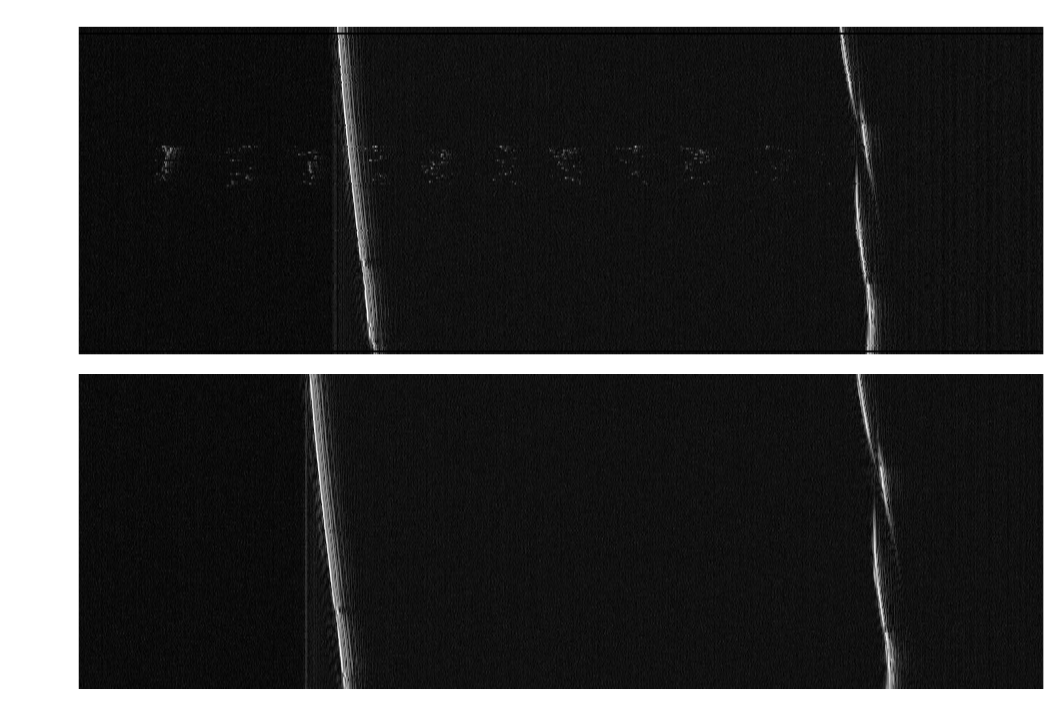
\includegraphics[width=0.8\textwidth]{rotterdam_02_water.png}
     \caption{30db}
   \label{fig:water_cavitation_70}
\end{figure}

\subsection{\Figref{water_cavitation_70}}
\subsubsection{General discussion of the image}
\Figref{water_cavitation_70} shows two plots.
Above is the B-mode for when both the driving wave and the imaging wave is on.
The two lines are the front and rear of the sample holder.
The lower plot is the same sample but when just the imaging wave is on.

In the top plot you can see banded specks that indicate the passage of the driving wave.  
%These are cavitation signals - you cannot make out the direct transmit in the image.
These signals are not present when the driving wave is off. % indicating that the signals are short lived (i.e. less than a few milliseconds - the time between adjacent A-lines).

At 30db suppression  such signals are fairly common but by no mean ubiquitous.
Often you get such signals only on a few A-lines (grouped together, as above) - sometimes only on 1 A-line - and often no signal at all.
At greater suppression (i.e 32 db) you get such signals but with much lesser frequency, maybe signal on some A-lines once in every 5 or 6 frames.
At lesser suppression they become more common.
The 30db signal has the property that you see  the bubbles at gains that  do not pick up the direct transmit.
This gives the images its `clean' appearance.

\subsubsection{Interpretation of the results}

\subsubsection{Quantifying Results}
A question that has not already been discussed could be  ``at what pressure does the cavitation signal manifest''.

The probabilistic nature of a cavitation is commonly overcome by asking for the pressure at which you 
generate a cavitation event in  50\% of the A-lines.
This approach was taken by Herbert\cite{Herbert2006} for the homogeneous nucleation of water.
Indeed, Herbert generated the probability density as a function of pressure.

However, it must be remembered that I am not doing homogeneous nucleation - 
the probability of a cavitation event is not a function of the water, 
but a function of its cleanliness and the degree to which the water is degassed.
So while I could plot a graph such as Herbert's, and quote a `threshold', I am not sure what this threshold would tell me?
Furthermore - since I am not {\em generating} a bubble (I am making an existing pocket of gas visible) - 
two separate A-lines are not independent. 
This invalidates the approach, and so any threshold I quote (of uncertain meaning) would be of dubious validity.

\todo[inline]{I cannot think of other relevant questions that I could ask of my data?}


\begin{figure}[h]
     \centering
          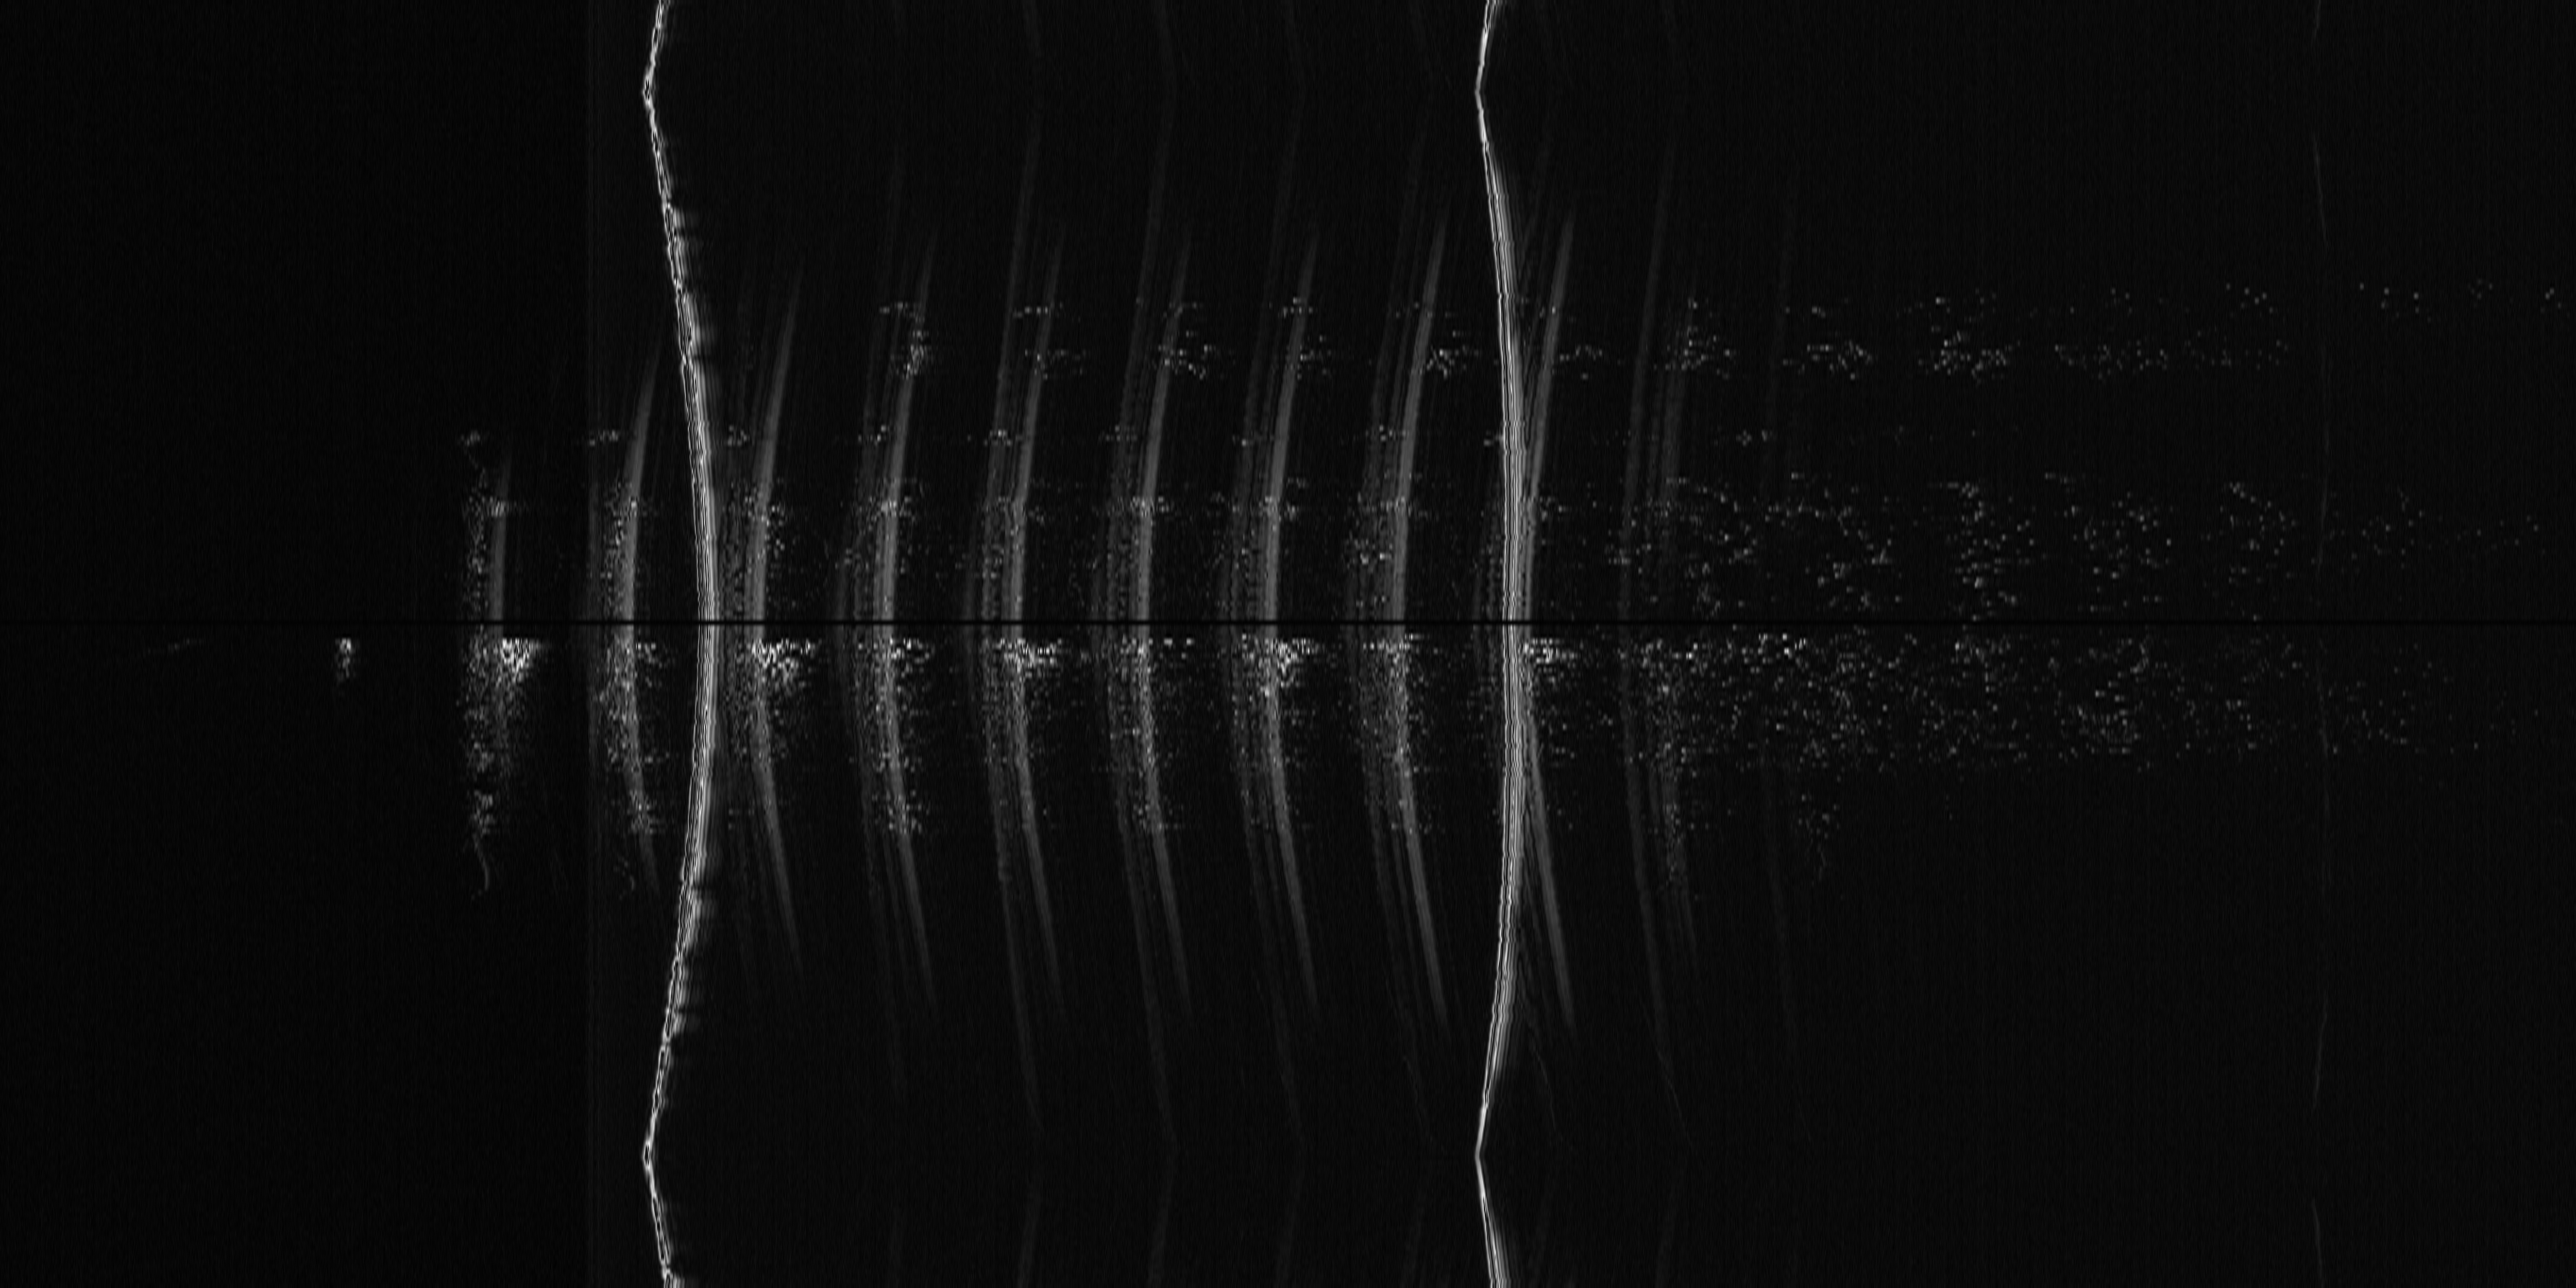
\includegraphics[width=0.8\textwidth]{C3water8500003.png}
     \caption{15db}
   \label{fig:water_cavitation_85}
\end{figure}


\subsection{\Figref{water_cavitation_85}}
\subsubsection{General discussion of the image}
The driving wave to \Figref{water_cavitation_85} has an applied voltage that is 15db greater than in \Figref{water_cavitation_70}.
You can clearly see the forward transmit, and various cavitation events throughout the B-mode image.

\subsubsection{The long tail of the image}
The problems in with the interpretation of this image are similar to the previous image (with the same solutions).
However, I include this image as I would like to draw your attention to what is in this image which is not in the previous.
In \figref{water_cavitation_85} I can count 16 bands in the signal, whereas in \figref{water_cavitation_70} I can count 10, possibly 11.
In both cases the signals were generated with a 10 electronic cycles. 
The difference between the two is presumably the degree of ringing in the driving transducer after the power has been turned off.
I have not done a beamplot for this pressure (John became a bit nervous about the cavitation events on the hydrophone).
However, the fact that you can see banding well after the signal finished suggests 
that you may see a response from the bubble even when the pressures from the driving transducer
are much reduced.

In these images, therefore, an addition interpretation is possible: that during the high pressure cycles 
the driving wave induces destructive cavitation of the bubbles - the bubbles grow and shrink and break with each cycle
(the stochastic nature of the images would support this, and at the high pressures such a result would not be a surprise)
but then in the  `ringing tail' periodic oscillation of a single stable bubble takes place. 
The test for the interaction between the two waves on a stable bubble would then be in the low pressure tail region.
This possibility was discussed in \chapref{mechanisms} and \chapref{experimental_method}.
The fact that periodic signals can be seen in this region is encouraging.
However, as before, without turning the imaging signal off it is impossible to say whether this result is actually interesting.


\section{Conclusion}
The problem that I have with the water cavitation experiments is that with the Cortex it is impossible to tell the mechanism  by which the cavitation event occurred.
If I am simply doing a passive detection of harmonic imaging then I don't believe my results contribute anything novel.
If it is more than harmonic imaging then my results, I believe, are interesting.
However, without turning off the imaging transducer it is impossible to answer this question.

This question cannot even be answered on the balance of probabilities.
This is because it would be very surprising if there was not any harmonic imaging present in the images.
It is therefore incumbent upon me, I believe, to demonstrate that there is not {\em just} harmonic imaging present.
The only way I can think of doing this is by subtracting away the contribution of the  driving wave. % (that is, pulse-inversion of the driving wave without the inversion).
This is difficult to do with the Cortex.
However, I believe it would be straight-forward in M-mode with the pulse-receive system that we now have available.




%\begin{figure}[h]
%     \centering
%          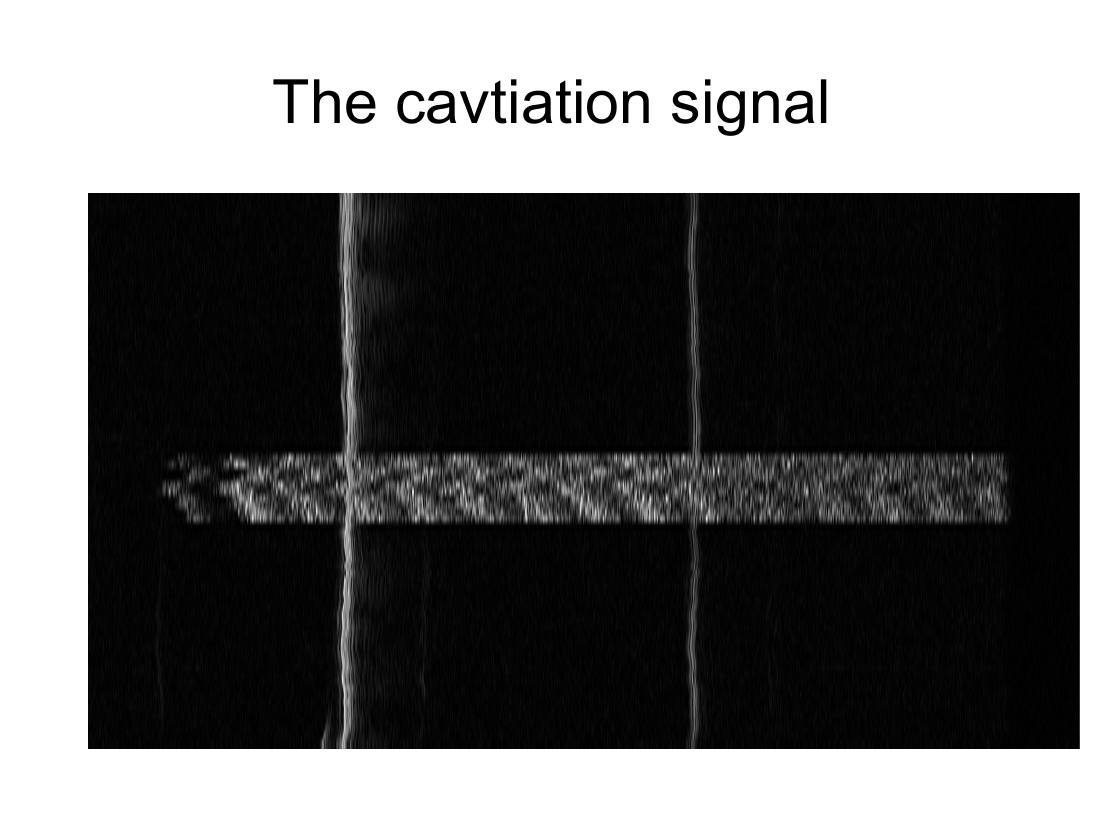
\includegraphics[width=0.8\textwidth]{emulsion_cavitation_signal.png}
%     \caption{Typical cavitation signal seen in bubbly water.
%     The two long vertical lines are the reflections of the sample
%     holder.
%     The imaging transducer is to the left,
%     the low-frequency transducer is to the right.}
%   \label{fig:cavitation}
%\end{figure}


%\begin{figure}[h]
%     \centering
%          
\includegraphics[width=0.8\textwidth]{pure90dbsmall41.png}
%     \caption{Typical cavitation signal seen in bubbly water.
%     The two long vertical lines are the reflections of the sample
%     holder.
%     The imaging transducer is to the left,
%     the low-frequency transducer is to the right.}
%   \label{fig:cavitation}
%\end{figure}



%%% Local Variables: 
%%% mode: latex
%%% TeX-master: "../../tshorrock_thesis"
%%% End: 

%  LocalWords:  Perfluorocarbon
